%%%%%%%%%%%%%%%%%%%%%%%%%%%%%%%%%%%%%%%%%%%%%%%%%%%%%%%%%%%%%%%
%%%  pta notes
%%%%%%%%%%%%%%%%%%%%%%%%%%%%%%%%%%%%%%%%%%%%%%%%%%%%%%%%%%%%%%%

\documentclass[onecolumn,fleqn,longbibliography]{revtex4}

% fonts
\usepackage{latexsym}
\usepackage{amsmath} 
\usepackage{amssymb} 
\usepackage{bm}
\usepackage{wasysym}

\usepackage{graphicx}


% extra by jarondl

\usepackage{array}
\usepackage{float}%unfloats
%\usepackage{multicol}
\usepackage[caption=false]{subfig} %subcaption is not compat with revtex
\usepackage[pdftitle={PTA},bookmarks]{hyperref}

%%%%%%%%%%%%%%%%%%%%%%%%%%%%%%%%%%%%%%%%%%%%%%%%%%%%%%%%%%%%%%%%

% NEW 
\newcommand{\abs}[1]{\left|#1\right|}
\newcommand{\varphiJ}{\bm{\varphi}}
\newcommand{\thetaJ}{\bm{\theta}}
%\renewcommand{\includegraphics}[2][0]{FIGURE}
\newcommand{\rmrk}[1]{\textcolor{red}{#1}}
\newcommand{\Eq}[1]{\textcolor{blue}{Eq.\!\!~(\ref{#1})}} 
\newcommand{\Fig}[1]{\textcolor{blue}{Fig.}\!\!~\ref{#1}}

% math symbols I
\newcommand{\sinc}{\mbox{sinc}}
\newcommand{\const}{\mbox{const}}
\newcommand{\trc}{\mbox{trace}}
\newcommand{\intt}{\int\!\!\!\!\int }
\newcommand{\ointt}{\int\!\!\!\!\int\!\!\!\!\!\circ\ }
\newcommand{\ar}{\mathsf r}
\newcommand{\im}{\mbox{Im}}
\newcommand{\re}{\mbox{Re}}

% math symbols II
\newcommand{\eexp}{\mbox{e}^}
\newcommand{\bra}{\left\langle}
\newcommand{\ket}{\right\rangle}

% Mass symbol
\newcommand{\mass}{\mathsf{m}} 
\newcommand{\rdisc}{\epsilon} 

% more math commands
\newcommand{\tbox}[1]{\mbox{\tiny #1}}
\newcommand{\bmsf}[1]{\bm{\mathsf{#1}}} 
\newcommand{\amatrix}[1]{\begin{matrix} #1 \end{matrix}} 
\newcommand{\pd}[2]{\frac{\partial #1}{\partial #2}}

% equations
\newcommand{\mylabel}[1]{\label{#1}} 
\newcommand{\beq}{\begin{eqnarray}}
\newcommand{\eeq}{\end{eqnarray}} 
\newcommand{\be}[1]{\begin{eqnarray}\ifthenelse{#1=-1}{\nonumber}{\ifthenelse{#1=0}{}{\mylabel{e#1}}}}
\newcommand{\ee}{\end{eqnarray}} 

% arrangement
\newcommand{\hide}[1]{}
\newcommand{\drawline}{\begin{picture}(500,1)\line(1,0){500}\end{picture}}
\newcommand{\bitem}{$\bullet$ \ \ \ }
\newcommand{\Cn}[1]{\begin{center} #1 \end{center}}
\newcommand{\mpg}[2][1.0\hsize]{\begin{minipage}[b]{#1}{#2}\end{minipage}}
\newcommand{\mpgt}[2][1.0\hsize]{\begin{minipage}[t]{#1}{#2}\end{minipage}}


%footnotemark:
\renewcommand*{\thefootnote}{\fnsymbol{footnote}}
%%%%%%%%%%%%%%%%%%%%%%%%%%%%%%%%%%%%%%%%%%%%%%%%%%%%%%%%%%%%%%%%%%%%%%%%%%%
% Sections
\newcommand{\sect}[1]
{
\addtocounter{section}{1} 
\setcounter{subsection}{0}
\ \\ 
\pdfbookmark[2]{\thesection. \ #1}{sect.\thesection}
{\Large\bf $=\!=\!=\!=\!=\!=\;$ [\thesection] \ #1}  
\nopagebreak
}

% subections
\newcommand{\subsect}[1]
{
\addtocounter{subsection}{1} 
\ \\ 
\pdfbookmark[2]{\ \ \ \ \thesection.\thesubsection. \ #1}{subsect.\thesection.\thesubsection}
{\bf $=\!=\!=\!=\!=\!=\;$ [\thesection.\thesubsection] \ #1}  
\nopagebreak
}
%%%%%%%%%%%%%%%%%%%%%%%%%%%%%%%%%%%%%%%%%%%%%%%%%%%%%%%%%%%%%%%%%%%%%%%%
%%%%%%%%%%%%%%%%%%%%%%%%%%%%%%%%%%%%%%%%%%%%%%%%%%%%%%%%%%%%%

\graphicspath{{figures/}}
\begin{document}

\title{PTA}

\author{YdL}

\maketitle

%%%%%%%%%%%%%%%%%%%%%%%%%%%%%%%%%%%%%%%%%%%%%%%%%%%%%%%%%%%%%%%%%%%%%%%%
%%%%%%%%%%%%%%%%%%%%%%%%%%%%%%%%%%%%%%%%%%%%%%%%%%%%%%%%%%%%%%%%%%%%%%%%

\sect{Introduction}

These are research notes regarding several aspects of random matrix spectrum,
in particular for banded matrices.

Our questions are what are the implications of several properties on the 
spectrum, and in particular:
\begin{itemize}
\item   If the disorder matrix is conservative (all row sums equal), 
        we have an ergodic mode , with $PN=N$. What about eigenmodes with
        eigenvalues close to the ergodic mode? can we predict their $PN$?
\item   If all matrix elements are positive, and the matrix is conservative,
        the eigenvalues are all positive, and the ergodic mode
        is at the edge of the spectrum. What if matrix elements are negative?
        where will the ergodic mode be? What is the meaning of a wide
        mode not in the minimal $\lambda$?
\item   What is the difference between diagonal disorder and banded disorder?
\item   How can we estimate the band position and $PN(\lambda)$, perhaps 
        with Anderson localization, and Thouless' formula?
\item   In the analysis of banded matrices, each $\lambda$ has more than 
        one or two corresponding velocities. Which velocity should we use?
\item   What about sparsity? In $1d$, sparsity makes the difference between
        diffusion and sub diffusion, because of percolative effects.
        What is the case for banded matrix?
        One assumption could be that banded disorder is similar
        to regular disorder with $s = b$.
\end{itemize}


%%%%%%%%%%%%%%%%%%%%%%%%%%%%%%%%%%%%%%%%%%%%%%%%%%%%%%%%%%%
\sect{Model}

We wish to study a banded model similar to the one presented in \cite{bodyfelt_scaling_2013},
starting with an ordered (and periodic) matrix:
%
\begin{align}\label{eq:ordered}
w_{nm} &= \begin{cases}
  w_0 &\qquad \textrm{ if  } \quad 0<|n-m|\le b \\
  0 &\qquad \textrm{ otherwise}
\end{cases}
\end{align}
%
According to Bloch's theorem, the eigenvectors of translational invariant
matrices are plane waves, and their eigenvalues can be easily deduced:
\begin{align}
k\ \  &=\ \  \frac{\pi m}{N} \ \ \ \ \ m=1..N \\
\vec{V}_k\ \  &=\ \  \cos(k\cdot x)\\
\lambda_k\ \  &=\ \  \sum_{n=1..b} 2\cos(n\cdot k) \\
&= \ \ -1 + \frac{\sin((b+\dfrac{1}{2})k)}{\sin(\dfrac{1}{2}k)}
\end{align}  
Where in the last step we have used one of Lagrange's trigonometric identities. 
The lower bound of $\lambda_k$ is $-2b$. 
$\lambda_k$ for several values of $b$ is plotted in \autoref{fig:theor_banded_ev}.

%%%%%%%%----------%%%%%%%%
%%%%%%%%  figure  %%%%%%%%
%%%%%%%%----------%%%%%%%%
\begin{figure}[H]
    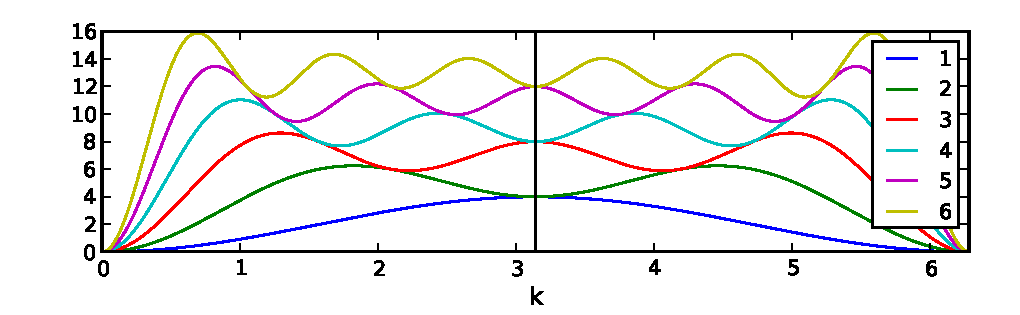
\includegraphics{pta_theor_banded_ev}
    \caption{$\lambda(k)$ for banded ordered matrices. Both plots
    represent the same curves, but in the left one there is a $+2b$ shift, both for clarity 
    and for later usage in conservative matrices. Since our 
    models are periodic, only the left half ($0,\pi$) of each plot is relevant. Since 
    the tangent is $DOS^{-1}$, the points with tangent zero are $DOS$ divergences.
    }
    \label{fig:theor_banded_ev}
\end{figure}



A cosine plane wave will have $PN= \frac{2}{3}N$. We can also compute the mode velocity:
\begin{align}
v \ \ &=\ \ \frac{d\lambda_k}{dk} \ \ =\ \ -\sum_{n=1..b} 2\cdot n\cdot \sin(n\cdot k)
\end{align}
Note that this expression is {\bf not single valued}. Meaning that each $\lambda$ 
has more than one associated velocity. 


The $DOS$ is defined by $\frac{dk}{d\lambda_k}$, which is the inverse of the 
velocity. Since density is additive, for each $\lambda$ we add the densities
of all relevant $k$ modes. For the moment we use a numerical solution to
find those $k$s. In \autoref{fig:dos} we plot the velocities and inverse 
$DOS$ as a function of $\lambda$.
%%%%%%%%----------%%%%%%%%
%%%%%%%%  figure  %%%%%%%%
%%%%%%%%----------%%%%%%%%
\begin{figure}[H]
    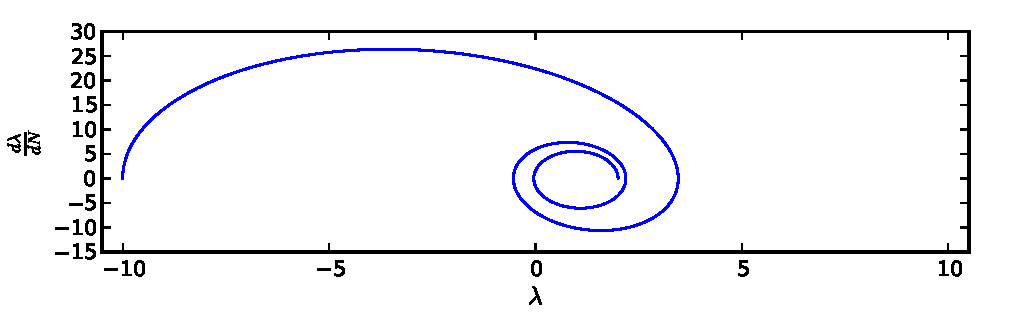
\includegraphics{pta_theor_banded_dos}
    \caption{The velocity and inverse $DOS$ for each eigenvalue $\lambda$, for $b=5$. 
             The inverse $DOS$ will always be less then the velocity. 
             We see large $DOS$ (small inverse) at energies where a single
             mode $DOS$ is diverging, and where we have more than one $k$.}
    \label{fig:dos}
\end{figure}


 
%%%%%%%%%%%%%%%%%%%%%%%%%%%%%%%%%%%%%%%%%%%%%%%%%%%%%
\sect{Adding disorder - finite localization}

The ordered lattice had no localization - all the $PN$ where equal to $\frac{2}{3}N$.
To study localization, we add to the ordered matrix $W_0$ a disordered matrix $V$:
%\renewcommand*{\thefootnote}{\fnsymbol{footnote}}
\begin{align}
W \ = \ W_0 \ + \ V
\end{align}
%
$W_0$ is the same banded matrix as before, with two parameters: $N$ and $b$.

$V$ is parametrized by a disorder parameter $\eta$, its own bandwidth $\tilde{b}$ 
(which can be different from $b$), and its conservativity. Later we
shall want to introduce a sparsity parameter $s$. 


The first kind of $V$ we examine has a uniformly distributed diagonal disorder:
\begin{align}
\gamma_n  \ = \  w_{nn} \ \in \ \left[-\frac{\eta}{2},+\frac{\eta}{2} \right]
\end{align}
{This disorder is not limited to positive elements},
which means that the spectrum is not bound.


This disorder, as small as it may be, will cause finite Anderson localization.
According to FGR, the transition rate (or the inverse of mean-free-time) is
\begin{align}
\frac{1}{t_\ell} = \varrho \langle w_{nm}^2\rangle
\end{align}
Where $\varrho$ is the Density-Of-States, and $w_{nm}$ is a rate between
neighboring sites.
To get the mean-free-path, we need to translate this to units of distance:
\begin{align}
\ell = v_\lambda t_\ell = \frac{v_\lambda}{\varrho \langle w_{nm}^2\rangle}
\end{align}
As mentioned before, the problem is that $v_\lambda$ is not single valued,
so we do not know yet what should be put there. If we put the inverse of 
the DOS, we get the expression:
\begin{align}
\ell = \frac{\varrho^{-2}}{ \langle w_{nm}^2\rangle}
\end{align}
We plot this result as a solid line in the next figures, with $<w^2> = \eta^2/3$.
On the eigenvalue axis, it does tell us about eigenvalues with low $PN$,
and the span (or band) where eigenvlaues exist. This does not scale with $N$, although 
the numerics seem to do so \autoref{fig:anderson_byN}

%%%%%%%%----------%%%%%%%%
%%%%%%%%  figure  %%%%%%%%
%%%%%%%%----------%%%%%%%%
\begin{figure}[H]
    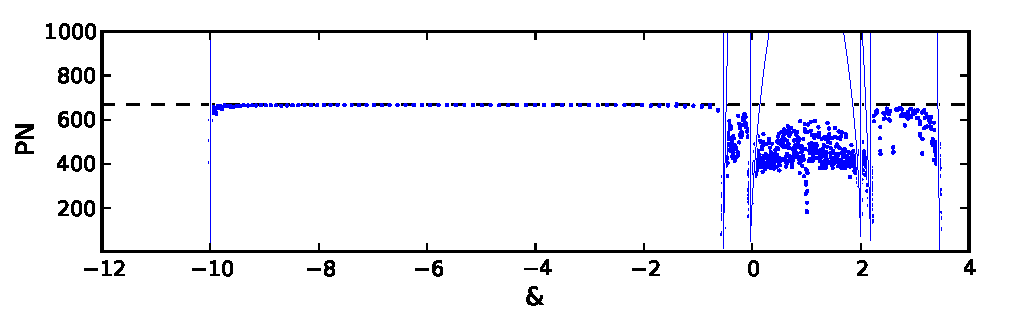
\includegraphics{pta_B_DD_low}\\
    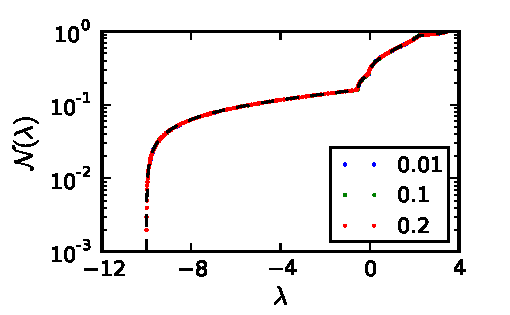
\includegraphics{pta_B_DD_low_ev}
    \caption{Top and bottom left: $PN$ vs eigenvalue $\lambda$, for $b=5$, $N=2000$. We see that
    no $PN$ is higher than the plane waves' $PN =2/3 N$. We can also explain
    points with low $PN$ by the corresponding $DOS$, and the band of eigenvalues. 
    Notice that there are eigenvalues below $-2b$. Also, there is a small unexplained bulge around $\lambda=1$.
    Compare this to figure 2 of \cite{bodyfelt_scaling_2013}.\protect\footnotemark Bottom right: cummulative distribution
    of the eigenvalues. The dashed black line is the theoretical expectation
    for an ordered matrix}
    \label{fig:ddonly_b5}
\end{figure}
%%%%%%%%%%%%%%%%%%%%%%%%%%%%%%%
\footnotetext{The 
    differences are that there the basic matrix (before disorder) had a 'conserving' diagonal of $-2b$,
    which corresponds to a horizontal shift, the $x$-axis there is $\sqrt{\lambda}$,
    the disorder is over the main $2b+1$ diagonal instead of only the main diagonal, 
    and the disorder is larger, $\eta=0.5$.}
    
    
%%%%%%%%----------%%%%%%%%
%%%%%%%%  figure  %%%%%%%%
%%%%%%%%----------%%%%%%%%
\begin{figure}[H]
    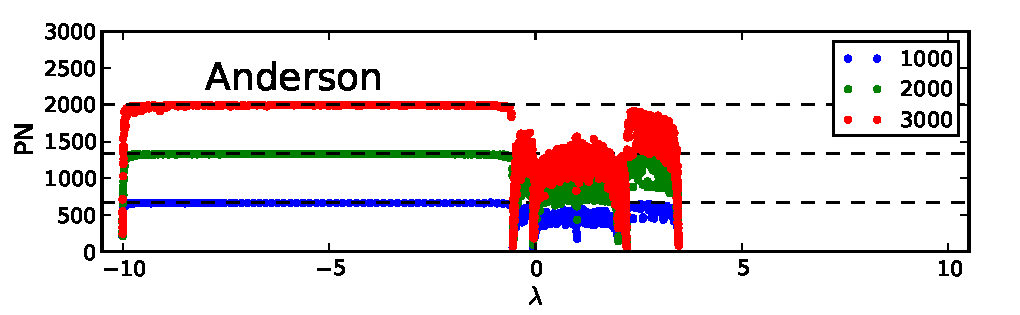
\includegraphics{pta_anderson_byN}
    \caption{$PN$ vs eigenvalue $\lambda$, for $b=5$, $\eta=0.1$ ,$N={{1000,2000,3000}}$. 
    Here we see the scaling in $N$ of the $PN$ values. The $PN$ of the 
    larger left portion scales as expected by $2/3 N$. In 
    \cite{bodyfelt_scaling_2013} this appears as the $PN>0.6N$ definition 
    of "extended modes". For this kind of disorder the other portion
    also scales in $N$, but less strongly. We assume that for a large enough
    $N$ the shape will converge to \autoref{fig:dos}, but that our sample
    size is not enough to show that fact. }
    \label{fig:anderson_byN}
\end{figure}


%%%%%%%%%%%%%%%%%%%%%%%%%%%%%%%%%%%%%%%%%%%%%%%%%%%%%%%%%%%%%%%%%%%%
\sect{Banded disorder}

Now we consider banded disorder. The $|m-n|\le b$ band has uniform disorder.
The positive version has uniform elements 
\begin{align} w_{nm} \in [0,2]\end{align}
, and the
symmetric version has 
\begin{align}w_{nm} \in [-2,2]\end{align}

%%%%%%%%----------%%%%%%%%
%%%%%%%%  figure  %%%%%%%%
%%%%%%%%----------%%%%%%%%
\begin{figure}[H]
    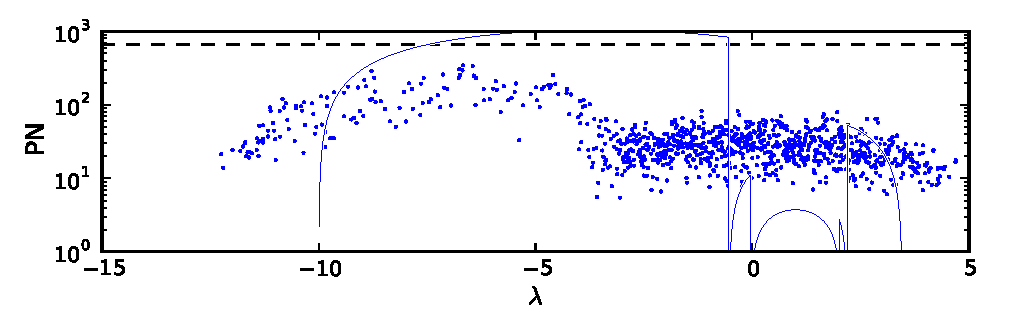
\includegraphics{pta_box2_positive}\\
    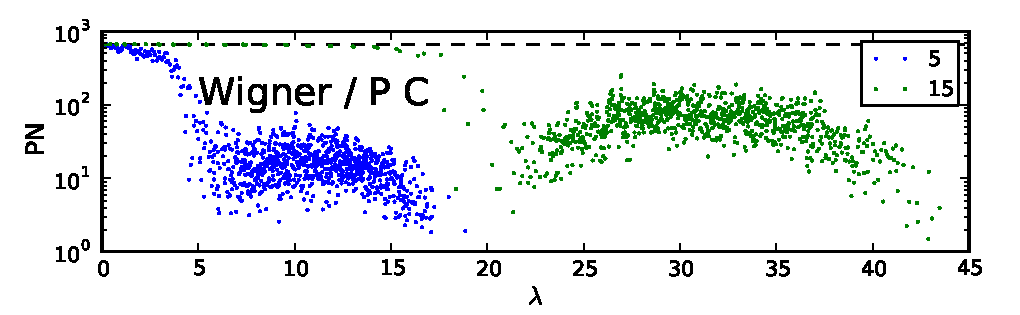
\includegraphics{pta_box2_pos_cons}\\
    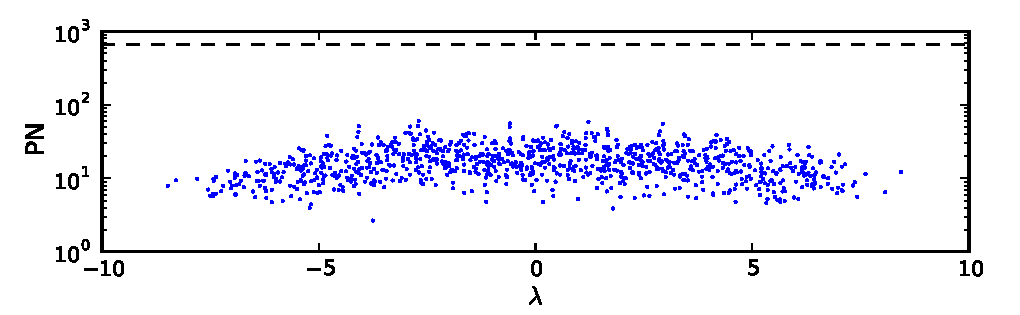
\includegraphics{pta_box2_symmetric}\\
    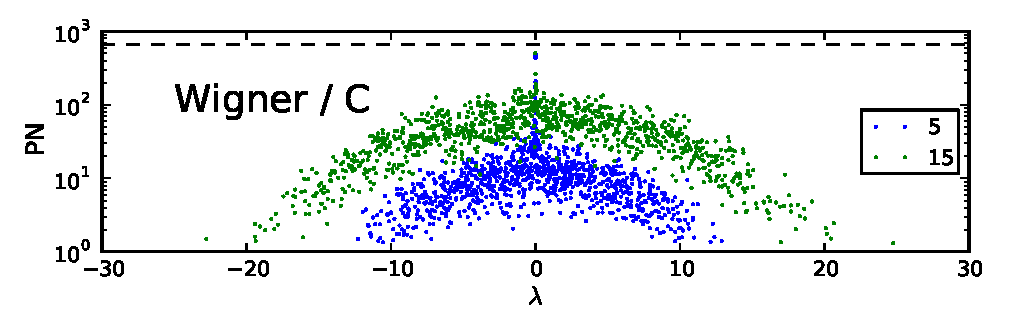
\includegraphics{pta_box2_sym_cons}
    \caption{$PN$ vs eigenvalue $\lambda$, for $b=5$, $N=1000$. From top to bottom:
    positive, positive and conserving, symmetric, symmetric and conserving. We see
    that the main effect of conservation is on the $\lambda=0$ modes. Note 
    that the x-axis is arbitrary, because we chose our limit at $2$ ($w_{nm} \in [0,2]$), but the 
    eigenvalues scale linearly in this limit without affecting the PN.
    The left branch we see depends only on $b$, and perhaps we can deduce its location
    from our previous analysis.}
    \label{fig:BB}
\end{figure}

%%%%%%%%%%%%%%%%%%%%%%%%%%%%%%%%%%%%%%%%%%%%%%%%%%%%%%%%%%%%%%%%%%%%%%%%
\sect{Band disorder, around a const}

In this model, the elements are taken from 
\begin{align} w_{nm} \in [\mu - \eta,\mu+\eta]\end{align}
The previous section matches $\mu=1, \quad \eta=1$. The model in \cite{bodyfelt_scaling_2013}
has $\mu=1, \quad \eta=\frac{1}{2}$. This introduces another dimensional-less
parameter besides $b$, $\frac{\eta}{\mu}$.

%%%%%%%%----------%%%%%%%%
%%%%%%%%  figure  %%%%%%%%
%%%%%%%%----------%%%%%%%%
\begin{figure}[H]
    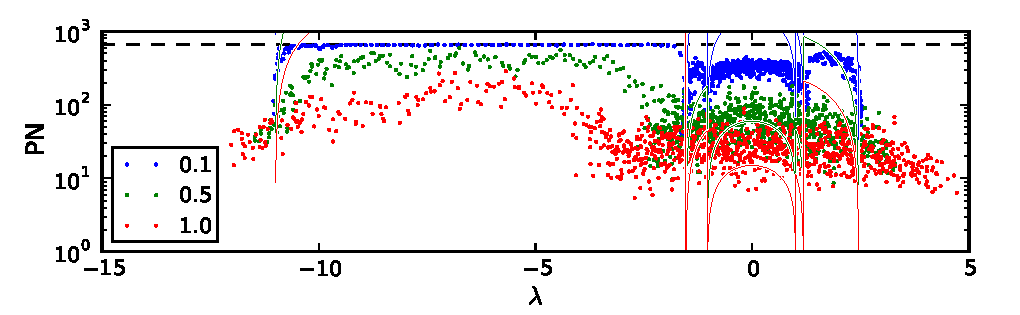
\includegraphics{pta_box_around1_positive}
    \caption{$PN$ vs eigenvalue $\lambda$, for $b=5$, $N=1000$, $\mu=1$ and changing $\eta$.
    We see the gradual shift from the known band structure.}
    \label{fig:box1}
\end{figure}
%%%%%%%%%%%%%%%%%%%%%%%%%%%%%%%%%%%%%%%%%%%%%%%%%%%%%%%%%%%%%%%%%%%%%%%%
\sect{Band exponential disorder (possibly sparse)}

We now consider a log-box model. 
\begin{align} w_{nm} \in \exp\left([- \eta,0]\right)\end{align}
%
For small $\eta$, this would be similar to the "Anderson" model,
while for large $\eta$ we have sparsity.

%%%%%%%%----------%%%%%%%%
%%%%%%%%  figure  %%%%%%%%
%%%%%%%%----------%%%%%%%%
\begin{figure}[H]
    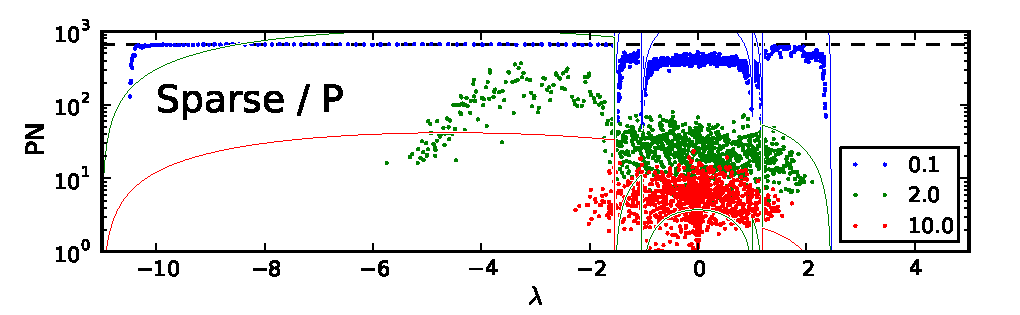
\includegraphics{pta_exp_regular}\\
    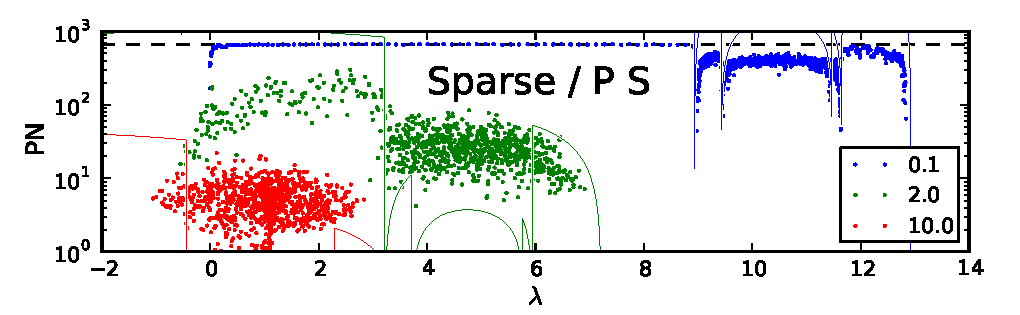
\includegraphics{pta_exp_shift}\\
    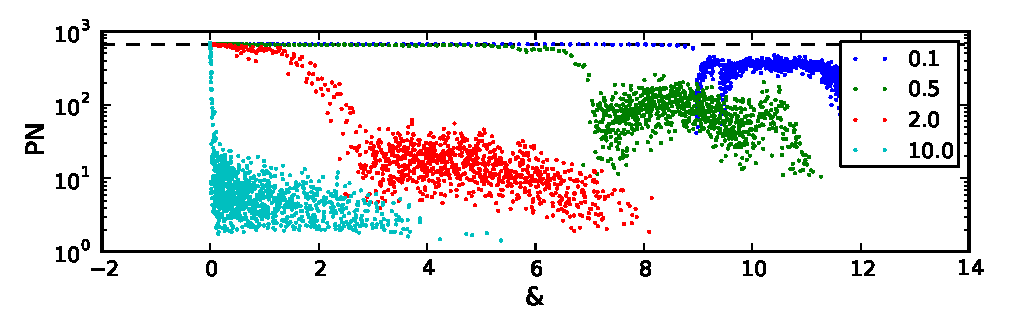
\includegraphics{pta_exp_cons}
    \caption{$PN$ vs eigenvalue $\lambda$, for $b=5$, $N=1000$, $\eta$ changing. 
    All three plots are for log-box distribution. The first is regular banded 
    log-box disorder. The second one contains shifts of the average row sum,
    $(2b+1)(1-e^{-\eta})/\eta$. The third one is conservative. }
    \label{fig:exp}
\end{figure}

\bibliographystyle{apsrev4-1}
\bibliography{../bibliography/jarondl,../bibliography/custom-longbib}


\end{document}
